
%% Harvard Physics Project
%% Test Booklet 6: The Nucleus
%%--------------------------------------------------


%% Test Booklet 6 contains 69 questions


%% Test A
%%--------------------
\element{project}{
\begin{question}{testA-Q01}
    %Questions 1, 2, and 3 refer to the following statement:
    An isotope of neon is represented by the symbol \ce{_{10}Ne^{21}}.
    How many electrons are there in a neutral atom of this isotope?
    \begin{multicols}{3}
    \begin{choices}
        \wrongchoice{\num{0}}
      \correctchoice{\num{10}}
        \wrongchoice{\num{11}}
        \wrongchoice{\num{21}}
        \wrongchoice{\num{31}}
        %% NOTE: added sixth for evenness
        \wrongchoice{\num{2}}
    \end{choices}
    \end{multicols}
\end{question}
}

\element{project}{
\begin{question}{testA-Q02}
    %Questions 1, 2, and 3 refer to the following statement:
    An isotope of neon is represented by the symbol \ce{_{10}Ne^{21}}.
    How many neutrons are in an atom of this isotope?
    \begin{multicols}{3}
    \begin{choices}
        \wrongchoice{\num{0}}
        \wrongchoice{\num{10}}
      \correctchoice{\num{11}}
        \wrongchoice{\num{21}}
        \wrongchoice{\num{31}}
        %% NOTE: added sixth for evenness
        \wrongchoice{\num{2}}
    \end{choices}
    \end{multicols}
\end{question}
}

\element{project}{
\begin{question}{testA-Q03}
    %Questions 1, 2, and 3 refer to the following statement:
    An isotope of neon is represented by the symbol \ce{_{10}Ne^{21}}.
    How many protons are in an atom of this isotope?
    \begin{multicols}{3}
    \begin{choices}
        \wrongchoice{\num{0}}
      \correctchoice{\num{10}}
        \wrongchoice{\num{11}}
        \wrongchoice{\num{21}}
        \wrongchoice{\num{31}}
        %% NOTE: added sixth for evenness
        \wrongchoice{\num{2}}
    \end{choices}
    \end{multicols}
\end{question}
}

\element{project}{
\begin{question}{testA-Q04}
    The charge-to-mass ratio of an alpha particle is the
        same as the charge-to-mass ratio of a:
    \begin{multicols}{2}
    \begin{choices}
        \wrongchoice{beta particle.}
        \wrongchoice{neutron.}
        \wrongchoice{proton.}
      \correctchoice{\ce{_{1}H^{2}} nucleus.}
        \wrongchoice{\ce{_{3}Li^{7}} nucleus.}
    \end{choices}
    \end{multicols}
\end{question}
}

\element{project}{
\begin{question}{testA-Q05}
    While looking for the emission of x-rays from fluorescent materials,
        Antoine Henri Becquerel discovered a new type of radiation.
    Which one of the following facts led Becquerel to suspect
        that the newly discovered rays were different from x-rays?
    \begin{choices}
      \correctchoice{The rays could penetrate thick black paper.}
        \wrongchoice{The rays were capable of producing ionizations in the air.}
        \wrongchoice{The rays were invisible to the naked eye.}
        \wrongchoice{The rays could not be started and stopped by the investigator.}
        \wrongchoice{The rays affected photographic plates.}
    \end{choices}
\end{question}
}

\element{project}{
\begin{question}{testA-Q06}
    Gamma rays are:
    \begin{choices}
      \correctchoice{high frequency electromagnetic radiation.}
        \wrongchoice{identical to electrons.}
        \wrongchoice{like electrons, but with a positive charge.}
        \wrongchoice{nuclei of the element helium.}
        \wrongchoice{neutral particles with mass number 1.}
    \end{choices}
\end{question}
}

\element{project}{
\begin{question}{testA-Q07}
    The major function of a cyclotron is:
    \begin{choices}
        \wrongchoice{to separate isotopes from one another.}
        \wrongchoice{to detect neutrons.}
        \wrongchoice{to produce neutrons.}
      \correctchoice{to accelerate charged particles.}
        \wrongchoice{to maintain a chain reaction.}
    \end{choices}
\end{question}
}

\element{project}{
\begin{question}{testA-Q08}
    Which one of the following processes is an example of nuclear fusion?
    \begin{choices}
        \wrongchoice{the formation of water from hydrogen and oxygen}
      \correctchoice{the formation of helium from hydrogen}
        \wrongchoice{the formation of barium and krypton from uranium}
        \wrongchoice{the formation of lead from radium by radioactive decay}
        \wrongchoice{the formation of potassium from potash}
    \end{choices}
\end{question}
}

\element{project}{
\begin{question}{testA-Q09}
    Over a period of time a certain radioactive atom emits the following
        particles in succession: alpha, alpha, beta, alpha, beta. \\[0.5\baselineskip]

    The atomic mass of the end product of this radioactive decay is
        less than the atomic mass of the original atom by approximately:
    \begin{multicols}{3}
    \begin{choices}
        \wrongchoice{\SI{1}{amu}.}
        \wrongchoice{\SI{3}{amu}.}
        \wrongchoice{\SI{6}{amu}.}
        \wrongchoice{\SI{10}{amu}.}
      \correctchoice{\SI{12}{amu}.}
    \end{choices}
    \end{multicols}
\end{question}
}

\element{project}{
\begin{question}{testA-Q10}
    Imagine that a new isotope of lithium with atomic number 3
        and mass number 5 has been discovered among the radiations
        emitted by radioactive plutonium.
    Which one of the following nuclear equations describes
        its emission from a \ce{_{94}Pu^{239}} nucleus?
    \begin{choices}
      \correctchoice{\ce{_{94}Pu^{239} -> _{3}Li^{5} + _{91}Pa^{234}}}
        \wrongchoice{\ce{_{94}PU^{239} -> _{3}Li^{5} + _{97}Bk^{244}}}
        \wrongchoice{\ce{_{94}PU^{239} -> _{3}Li^{5} + _{91}Pa^{244}}}
        \wrongchoice{\ce{_{94}PU^{239} -> _{5}Li^{3} + _{89}Pa^{236}}}
        \wrongchoice{\ce{_{94}PU^{239} -> _{5}Li^{3} + _{91}Pa^{234}}}
    \end{choices}
\end{question}
}

\element{project}{
\begin{question}{testA-Q11}
    A standard way of representing a given nuclide of element $X$ is \ce{_{Z}X^{A}}.
    Which of the following symbols can minimally identify the nuclide completely?
    \begin{multicols}{2}
    \begin{choices}
        \wrongchoice{A only}
        \wrongchoice{X only}
        \wrongchoice{X and Z only}
      \correctchoice{A and Z only}
        \wrongchoice{A, X and Z}
    \end{choices}
    \end{multicols}
\end{question}
}

\element{project}{
\begin{question}{testA-Q12}
    The chemical properties of an atom are determined by its:
    \begin{choices}
        \wrongchoice{mass number.}
        \wrongchoice{number of isotopes.}
      \correctchoice{atomic number.}
        \wrongchoice{nuclear binding energy.}
    \end{choices}
\end{question}
}

\element{project}{
\begin{question}{testA-Q13}
    A proton of mass $m_p$ and a neutron of mass $m_n$ combine
        in a fusion process to form a stable deuterium nucleus.
    The mass of this nucleus is:
    \begin{choices}
        \wrongchoice{greater than $m_p$ plus $m_n$.}
        \wrongchoice{equal to $m_p$ plus $m_n$.}
      \correctchoice{less than $m_p$ plus $m_n$.}
        \wrongchoice{sometimes less than and sometimes equal to $m_p$ plus $m_n$.}
        \wrongchoice{sometimes greater than and sometimes equal to $m_n$.}
    \end{choices}
\end{question}
}

\element{project}{
\begin{question}{testA-Q14}
    According to the proton-neutron theory of the atomic nucleus,
        beta-particle emission results from:
    \begin{choices}
        \wrongchoice{a proton changing into an alpha particle.}
      \correctchoice{a neutron changing into a proton.}
        \wrongchoice{a proton expelling an electron from the electron shells of the atom.}
        \wrongchoice{a gamma ray producing an electron and positron.}
        \wrongchoice{the loss of one of the electrons in the nucleus.}
    \end{choices}
\end{question}
}

\element{project}{
\begin{question}{testA-Q15}
    The purpose of a moderator in an atomic reactor is to:
    \begin{choices}
        \wrongchoice{provide neutrons for the fission process.}
        \wrongchoice{react with the uranium to release energy.}
      \correctchoice{slow down fast neutrons to increase the probability of fission.}
        \wrongchoice{absorb the dangerous gamma radiation.}
    \end{choices}
\end{question}
}


%% Test B
%%--------------------
\element{project}{
\begin{question}{testB-Q01}
    Biologists are learning more about the metabolism
        of plants and animals through the use of:
    \begin{choices}
        \wrongchoice{high-energy particle accelerators.}
        \wrongchoice{cloud-chamber photography.}
      \correctchoice{isotopic tracers.}
        \wrongchoice{mass spectroscopy.}
        \wrongchoice{cosmic rays.}
    \end{choices}
\end{question}
}

\element{project}{
\begin{question}{testB-Q02}
    Alpha particles:
    \begin{choices}
        \wrongchoice{are electromagnetic radiation of high frequency.}
        \wrongchoice{are negatively charged particles.}
        \wrongchoice{have the highest penetrating power of the three types of radiation emitted by radioactive elements.}
      \correctchoice{produce the greatest amount of ionization per centimeter of the three kinds of emissions from radioactive nuclei.}
        \wrongchoice{have the same properties as electrons.}
    \end{choices}
\end{question}
}

\element{project}{
\begin{questionmult}{testB-Q03}
    Which of the following is (are) true of beta particles?
    \begin{choices}
      \correctchoice{They originate from atomic nuclei.}
        \wrongchoice{They have the same properties as electrons.}
      \correctchoice{If they travel through air, they produce ionization.}
    \end{choices}
\end{questionmult}
}

\element{project}{
\begin{question}{testB-Q04}
    The electron volt (\si{\eV}) is a unit of:
    \begin{multicols}{2}
    \begin{choices}
      \correctchoice{energy.}
        \wrongchoice{speed.}
        \wrongchoice{voltage.}
        \wrongchoice{radioactivity}
        \wrongchoice{force.}
    \end{choices}
    \end{multicols}
\end{question}
}

\element{project}{
\begin{question}{testB-Q05}
    Which graph best represents the change with time of the
        amount of stable lead present in a sample that was originally pure uranium 238?
    \begin{multicols}{2}
    \begin{choices}
        \AMCboxDimensions{down=-3.5em}
        \wrongchoice{
            \begin{tikzpicture}
                \begin{axis}[
                    axis y line=left,
                    axis x line=bottom,
                    axis line style={->},
                    xlabel={time},
                    x unit=\SI{e9}{year},
                    xtick={0,5,10,15},
                    ylabel={amount of lead},
                    ytick=\empty,
                    xmin=0,xmax=16,
                    ymin=0,ymax=16,
                    width=1.00\columnwidth,
                    very thin,
                ]
                \addplot[line width=1pt,domain=0:15]{sqrt(15)*sqrt(x)};
                \end{axis}
            \end{tikzpicture}
        }
        \wrongchoice{
            \begin{tikzpicture}
                \begin{axis}[
                    axis y line=left,
                    axis x line=bottom,
                    axis line style={->},
                    xlabel={time},
                    x unit=\SI{e9}{year},
                    xtick={0,5,10,15},
                    ylabel={amount of lead},
                    ytick=\empty,
                    xmin=0,xmax=16,
                    ymin=0,ymax=16,
                    width=1.00\columnwidth,
                    very thin,
                ]
                \addplot[line width=1pt,domain=0:15]{0.06*x*x};
                \end{axis}
            \end{tikzpicture}
        }
        %% NOTE: exponetial decay
        \correctchoice{
            \begin{tikzpicture}
                \begin{axis}[
                    axis y line=left,
                    axis x line=bottom,
                    axis line style={->},
                    xlabel={time},
                    x unit=\SI{e9}{year},
                    xtick={0,5,10,15},
                    ylabel={amount of lead},
                    ytick=\empty,
                    xmin=0,xmax=16,
                    ymin=0,ymax=16,
                    width=1.00\columnwidth,
                    very thin,
                ]
                \addplot[line width=1pt,domain=0:15]{15*exp(-0.15*x)};
                \end{axis}
            \end{tikzpicture}
        }
        \wrongchoice{
            \begin{tikzpicture}
                \begin{axis}[
                    axis y line=left,
                    axis x line=bottom,
                    axis line style={->},
                    xlabel={time},
                    x unit=\SI{e9}{year},
                    xtick={0,5,10,15},
                    ylabel={amount of lead},
                    ytick=\empty,
                    xmin=0,xmax=16,
                    ymin=0,ymax=16,
                    width=1.00\columnwidth,
                    very thin,
                ]
                \addplot[line width=1pt,domain=0:15]{15-0.95*x};
                \end{axis}
            \end{tikzpicture}
        }
        \wrongchoice{
            \begin{tikzpicture}
                \begin{axis}[
                    axis y line=left,
                    axis x line=bottom,
                    axis line style={->},
                    xlabel={time},
                    x unit=\SI{e9}{year},
                    xtick={0,5,10,15},
                    ylabel={amount of lead},
                    ytick=\empty,
                    xmin=0,xmax=16,
                    ymin=0,ymax=16,
                    width=1.00\columnwidth,
                    very thin,
                ]
                \addplot[line width=1pt,domain=0:15]{x};
                \end{axis}
            \end{tikzpicture}
        }
    \end{choices}
    \end{multicols}
\end{question}
}

\element{project}{
\begin{question}{testB-Q06}
    \emph{All except one} of the following particles can be
        accelerated by an electric or magnetic field.
    Which one is the exception?
    \begin{choices}
        \wrongchoice{electron}
        \wrongchoice{proton}
      \correctchoice{neutron}
        \wrongchoice{alpha particle}
        \wrongchoice{deuteron (\ce{_{1}H^{2}} nucleus)}
    \end{choices}
\end{question}
}

\element{project}{
\begin{question}{testB-Q07}
    %Questions 7 and 8 list key discoveries in the field of nuclear physics.
    %From the list below, select the person most responsible for the discovery.
    Select the scientist most responsible for the discovery of radium.
    \begin{choices}
        \wrongchoice{Antoine Henri Becquerel}
      \correctchoice{Marie Sk{\l}odowska-Curie}
        \wrongchoice{Frederick Soddy}
        \wrongchoice{James Chadwick}
        \wrongchoice{Enrico Fermi}
    \end{choices}
\end{question}
}

\element{project}{
\begin{question}{testB-Q08}
    Select the scientist most responsible for the discovery of the neutron.
    \begin{choices}
        \wrongchoice{Antoine Henri Becquerel}
        \wrongchoice{Marie Sk{\l}odowska-Curie}
        \wrongchoice{Frederick Soddy}
      \correctchoice{James Chadwick}
        \wrongchoice{Enrico Fermi}
    \end{choices}
\end{question}
}

\element{project}{
\begin{question}{testB-Q09}
    Isotopes of an element have:
    \begin{choices}
        \wrongchoice{different masses and different atomic numbers.}
      \correctchoice{the same chemical properties but different masses.}
        \wrongchoice{the same chemical properties but different atomic numbers.}
        \wrongchoice{the same mass but different atomic numbers.}
        \wrongchoice{the same atomic number but different chemical properties.}
    \end{choices}
\end{question}
}

\element{project}{
\begin{questionmult}{testB-Q10}
    The law of decay of radioactive samples is a statistical law.
    This implies that:
    \begin{choices}
      \correctchoice{it is only applicable to samples containing a large number of atoms.}
      \correctchoice{it can predict little about the time of decay of an individual atom.}
      \correctchoice{it makes no assumptions as to why atoms disintegrate.}
    \end{choices}
\end{questionmult}
}

%% NOTE: duplicate of testC-Q28
\element{project}{
\begin{question}{testB-Q11}
    Select the equation that represents the formation of a transuranium element.
    \begin{choices}
        \wrongchoice{\ce{_{0}n^{1} + _{94}Pu^{239} -> _{56}Ba^{141} + _{38}Sr^{96} + 3_{0}n^{1}}}
        \wrongchoice{\ce{4_{1}H^{1} -> _{2}He^{4} + 2_{+1}e^{0} + 2\nu + \gamma}}
      \correctchoice{\ce{_{0}n^{1} + _{92}Pu^{238} -> _{92}U^{239}}; \\[1em]
                     \ce{_{92}U^{239} -> _{93}Np^{239} + _{-1}e^{0} + \nu}}
        \wrongchoice{\ce{_{0}n^{1} + _{13}Al^{27} -> _{13}Al^{28}}}
        \wrongchoice{\ce{_{1}H^{2} + _{80}Hg^{199} -> _{79}Au^{197} + _{2}He^{4}}}
    \end{choices}
\end{question}
}

%% NOTE: duplicate of testC-Q29
\element{project}{
\begin{question}{testB-Q12}
    Select the equation that represents the release of energy in stars.
    \begin{choices}
        \wrongchoice{\ce{_{0}n^{1} + _{94}Pu^{239} -> _{56}Ba^{141} + _{38}Sr^{96} + 3_{0}n^{1}}}
      \correctchoice{\ce{4_{1}H^{1} -> _{2}He^{4} + 2_{+1}e^{0} + 2\nu + \gamma}}
        \wrongchoice{\ce{_{0}n^{1} + _{92}Pu^{238} -> _{92}U^{239}};  \\[1em]
                     \ce{_{92}U^{239} -> _{93}Np^{239} + _{-1}e^{0} + \nu}}
        \wrongchoice{\ce{_{0}n^{1} + _{13}Al^{27} -> _{13}Al^{28}}}
    \end{choices}
\end{question}
}

\element{project}{
\begin{question}{testB-Q13}
    In 1939, Hahn and Strassman identified barium as one of the
        disintegration products produced when uranium was bombarded with neutrons.
    The importance of this discovery was that it suggested that:
    \begin{choices}
      \correctchoice{the nucleus of the uranium atom could be split apart.}
        \wrongchoice{the uranium atom is really several barium atoms bound together.}
        \wrongchoice{uranium could be made radioactive.}
        \wrongchoice{uranium and barium were isotopes of the same element.}
        \wrongchoice{neutrons were converted into barium atoms.}
    \end{choices}
\end{question}
}

\element{project}{
\begin{question}{testB-Q14}
    Rutherford identified three types of radiation emitted from radium: alpha, beta, and gamma.
    If these radiations are listed in order of increasing penetrating power,
        with the least penetrating listed first, the order is:
    \begin{choices}
      \correctchoice{alpha, beta, gamma.}
        \wrongchoice{beta, gamma, alpha.}
        \wrongchoice{gamma, alpha, beta.}
        \wrongchoice{beta, alpha, gamma.}
        \wrongchoice{alpha, gamma, beta.}
    \end{choices}
\end{question}
}

%% NOTE: near duplicate of testA-Q15
\element{project}{
\begin{question}{testB-Q15}
    The purpose of a moderator in an atomic reactor is to:
    \begin{choices}
        \wrongchoice{provide neutrons for the fission process.}
        \wrongchoice{react with the uranium to release energy.}
      \correctchoice{slow down fast neutrons to increase the probability of fission.}
        \wrongchoice{release energy by combustion to keep the reactor ``critical.''}
        \wrongchoice{absorb the dangerous gamma radiation.}
    \end{choices}
\end{question}
}


%% Test C
%%--------------------
\element{project}{
\begin{question}{testC-Q01}
    %Questions 1, 2, and 3 refer to the following statement:
    An isotope of neon is represented by the symbol \ce{_{6}Ne^{13}}.
    How many electrons are there in a neutral atom of this isotope?
    \begin{multicols}{3}
    \begin{choices}
        \wrongchoice{\num{0}}
      \correctchoice{\num{6}}
        \wrongchoice{\num{7}}
        \wrongchoice{\num{13}}
        \wrongchoice{\num{19}}
        %% NOTE: added for evenness
        \wrongchoice{\num{2}}
    \end{choices}
    \end{multicols}
\end{question}
}

\element{project}{
\begin{question}{testC-Q02}
    An isotope of neon is represented by the symbol \ce{_{6}C^{13}}.
    How many protons are there in a neutral atom of this isotope?
    \begin{multicols}{3}
    \begin{choices}
        \wrongchoice{\num{0}}
      \correctchoice{\num{6}}
        \wrongchoice{\num{7}}
        \wrongchoice{\num{13}}
        \wrongchoice{\num{19}}
        %% NOTE: added for evenness
        \wrongchoice{\num{2}}
    \end{choices}
    \end{multicols}
\end{question}
}

\element{project}{
\begin{question}{testC-Q03}
    An isotope of neon is represented by the symbol \ce{_{6}C^{13}}.
    How many neutrons are there in a neutral atom of this isotope?
    \begin{multicols}{3}
    \begin{choices}
        \wrongchoice{\num{0}}
        \wrongchoice{\num{6}}
      \correctchoice{\num{7}}
        \wrongchoice{\num{13}}
        \wrongchoice{\num{19}}
        %% NOTE: added for evenness
        \wrongchoice{\num{2}}
    \end{choices}
    \end{multicols}
\end{question}
}

\element{project}{
\begin{question}{testC-Q04}
    The charge on a proton is expressed in:
    \begin{multicols}{2}
    \begin{choices}
        \wrongchoice{amperes (\si{\ampere}).}
      \correctchoice{coulombs (\si{\coulomb}).}
        \wrongchoice{electron volts (\si{\eV}).}
        \wrongchoice{ohms (\si{\ohm}).}
        \wrongchoice{joules (\si{\joule}).}
    \end{choices}
    \end{multicols}
\end{question}
}

\element{project}{
\begin{question}{testC-Q05}
    Radioactive bismuth has a half-life of 5 days.
    A \SI{1}{\gram} sample of bismuth is prepared.
    After 5 days,
        the amount of bismuth in the sample is very close to:
    \begin{multicols}{3}
    \begin{choices}
        \wrongchoice{\SI{1/16}{\gram}}
        \wrongchoice{\SI{1/8}{\gram}}
        \wrongchoice{\SI{1/4}{\gram}}
      \correctchoice{\SI{1/2}{\gram}}
        \wrongchoice{\SI{1}{\gram}}
    \end{choices}
    \end{multicols}
\end{question}
}

\element{project}{
\begin{question}{testC-Q06}
    \emph{All except one} of the following statements are true.
    Which one is the exception?
    \begin{choices}
        \wrongchoice{Radioactivity is a natural characteristic of some elements.}
        \wrongchoice{Radioactive isotopes can be produced in the laboratory.}
        \wrongchoice{Radioactive isotopes decay by the emission of particles from the nucleus.}
      \correctchoice{All isotopes are radioactive.}
        \wrongchoice{There is a wide variety of decay rates for radioactive elements.}
    \end{choices}
\end{question}
}

\element{project}{
\begin{question}{testC-Q07}
    Three of the names listed below refer to the same thing.
    Which one does \emph{not}?
    \begin{multicols}{2}
    \begin{choices}
        \wrongchoice{electrons}
        \wrongchoice{beta particles}
        \wrongchoice{cathode rays}
      \correctchoice{alpha particles}
    \end{choices}
    \end{multicols}
\end{question}
}

\element{project}{
\begin{question}{testC-Q08}
    The radiation from a sample of \ce{Kr^{85}} decreases to
        one-third of the original intensity $I_0$ in a period of 18 years.
    What would be the intensity after 18 \emph{more} years.
    \begin{multicols}{3}
    \begin{choices}
        \wrongchoice{$I_0$}
        \wrongchoice{$\dfrac{1}{2} I_0$}
        \wrongchoice{$\dfrac{1}{3} I_0$}
        \wrongchoice{$\dfrac{1}{6} I_0$}
      \correctchoice{$\dfrac{1}{9} I_0$}
    \end{choices}
    \end{multicols}
\end{question}
}

\element{project}{
\begin{question}{testC-Q09}
    Suppose that a new type of radiation, the $T$ particle,
        is discovered among the radiations emitted by certain elements.
    Suppose measurements yield the following information:
    \begin{enumerate}
        \item The charge-to-mass ratio of the $T$ particle is one-third that of the charge-to-mass ratio of a proton.
        \item $T$ particles are deflected in a magnetic field in the same direction as alpha particles.
    \end{enumerate}
    Which one of the following symbols could describe the particle?
    \begin{multicols}{3}
    \begin{choices}
        \wrongchoice{\ce{_{-1/3}T^{1}}}
        \wrongchoice{\ce{_{-1}T^{3}}}
      \correctchoice{\ce{_{1}T^{3}}}
        \wrongchoice{\ce{_{-3}T^{1}}}
        \wrongchoice{\ce{_{3}T^{1}}}
    \end{choices}
    \end{multicols}
\end{question}
}

\element{project}{
\begin{question}{testC-Q10}
    Rutherford identified three types of radiation emitted
        from radium: alpha, beta, and gamma.
    If these radiations are listed in order of increasing
        penetrating power, with the least penetrating radiation
        listed first, the order is
    \begin{choices}
      \correctchoice{alpha, beta, gamma.}
        \wrongchoice{beta, gamma, alpha.}
        \wrongchoice{gamma, alpha, beta.}
        \wrongchoice{beta, alpha, gamma.}
        \wrongchoice{alpha, gamma, beta.}
    \end{choices}
\end{question}
}

%\element{project}{
%\begin{question}{testC-Q11}
%    %Question 11 refers to the following information:
%    An isotope of polonium is gradually transmuted to lead
%        according to the following decay scheme
%    (the half -life for each member is listed below its symbol).
%    %% NOTE: TODO: Make multiline
%    \begin{align*}
%        \ce{Po^{218}} &\rightarrow
%        \ce{Pb^{214}} &\rightarrow
%        \ce{Bi^{214}} &\rightarrow
%        \ce{Po^{214}} &\rightarrow
%        \ce{Pb^{210}} &\rightarrow
%        \ce{Bi^{210}} &\rightarrow
%        \ce{Po^{210}} &\rightarrow
%        \ce{Pb^{206}} \\
%        \SI{3.05}{\minute} &
%        \SI{26.8}{\minute} &
%        \SI{19.7}{\minute} &
%        \SI{1.6e-4}{\second} &
%        \SI{21.4}{\year} &
%        \SI{5.0}{\day} &
%        \SI{138.4}{\day} &
%        \text{stable} \\
%    \end{align*}
%    If we have a pure sample of \ce{Po^{218}} initially,
%        which member of the series will be present in the
%        greatest amount after one day?
%    \begin{multicols}{3}
%    \begin{choices}
%        \wrongchoice{\ce{Pb^{206}}}
%        \wrongchoice{\ce{Po^{210}}}
%      \correctchoice{\ce{Pb^{210}}}
%        \wrongchoice{\ce{Bi^{214}}}
%        \wrongchoice{\ce{Pb^{214}}}
%    \end{choices}
%    \end{multicols}
%\end{question}
%}

\element{project}{
\begin{question}{testC-Q12}
    \emph{All except one} of the following particles
        leaves a track of condensed vapor when is passes
        through a cloud chamber.
    Which one is the exception?
    \begin{multicols}{2}
    \begin{choices}
        \wrongchoice{electron}
      \correctchoice{neutron}
        \wrongchoice{positron}
        \wrongchoice{alpha particle}
        \wrongchoice{proton}
    \end{choices}
    \end{multicols}
\end{question}
}

\element{project}{
\begin{questionmult}{testC-Q13}
    Assume you know nothing about the rays from a radioactive isotope except that,
        in a uniform magnetic field, they behave as shown in the diagram below.
    \begin{center}
    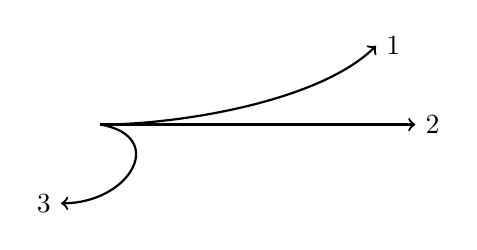
\begin{tikzpicture}
        %\draw[thick,->] (0,0) to[out=15,in=230,looseness=0.5] (3,1) node[anchor=west] {1};
        \draw[thick,->] (0,0) to[controls=+(0:1) and +(-135:1)] (3.5,1) node[anchor=west] {1};
        \draw[thick,->] (0,0) -- (4,0) node[anchor=west] {2};
        \draw[thick,->] (0,0) to[out=350,in=0,looseness=2.0] (-0.5,-1) node[anchor=east] {3};
    \end{tikzpicture}
    \end{center}
    (The magnetic field is directed into the paper.)
    Which one of the following statements \emph{must} be true about the rays which move along paths 1, 2 and 3?
    \begin{choices}
      \correctchoice{3 has a charge of larger magnitude than 2.}
        \wrongchoice{1 consists of electromagnetic radiation.}
        \wrongchoice{The speed of 3 is different from that of 2.}
        \wrongchoice{3 consists of particles of smaller mass than 2.}
      \correctchoice{1 and 3 both consist of charged particles.}
    \end{choices}
\end{questionmult}
}

\element{project}{
\begin{question}{testC-Q14}
    Which one of the following is true of the most stable nuclides?
    They have:
    \begin{choices}
      \correctchoice{even numbers of protons and neutrons.}
        \wrongchoice{odd numbers of protons and neutrons.}
        \wrongchoice{even numbers of protons, odd numbers of neutrons.}
        \wrongchoice{odd numbers of protons, even numbers of neutrons.}
        \wrongchoice{equal numbers of protons and neutrons, regardless of whether odd or even.}
    \end{choices}
\end{question}
}

\element{project}{
\begin{question}{testC-Q15}
    Nuclide $A$ decays by emitting a beta particle and forms nuclide $B$.
    Compared to nuclide $A$, nuclide $B$ has:
    \begin{choices}
      \correctchoice{a charge of one unit more, and practically the same mass.}
        \wrongchoice{a charge of one unit more, and a mass one unit less.}
        \wrongchoice{a charge of one unit less, and a mass one unit more.}
        \wrongchoice{a charge of one unit less, and a mass one unit less.}
        \wrongchoice{a charge of one unit less, and a mass two units less.}
    \end{choices}
\end{question}
}

\element{project}{
\begin{question}{testC-Q16}
    Which of the following pairs of nuclei are isotopes of the same element?
    \begin{choices}
        \wrongchoice{two nuclei with the same numbers of neutrons, but different numbers of protons}
        \wrongchoice{a nucleus of carbon and a nucleus of nitrogen, both nuclei with the same mass}
        \wrongchoice{two nuclei that carry different electric charges, but have the same mass}
        \wrongchoice{two nuclei in which the number of protons equals the number of neutrons}
      \correctchoice{two nuclei that have the same numbers of protons, but with different masses}
    \end{choices}
\end{question}
}

\element{project}{
\begin{question}{testC-Q17}
    \emph{All except one} of the following particles can be
        accelerated by an electric or magnetic field.
    Which one is the exception!
    \begin{choices}
        \wrongchoice{electron}
        \wrongchoice{proton}
      \correctchoice{neutron}
        \wrongchoice{alpha particle}
        \wrongchoice{deuteron (\ce{_{1}H^{2}} nucleus)}
    \end{choices}
\end{question}
}

\element{project}{
\begin{question}{testC-Q18}
    An atom of mass number 11 and atomic number 5 captures
        an alpha particle and then emits a proton.
    The mass number of the resulting atom will be:
    \begin{multicols}{3}
    \begin{choices}
        \wrongchoice{10}
        \wrongchoice{11}
        \wrongchoice{12}
        \wrongchoice{13}
      \correctchoice{14}
        %% NOTE: add one for evenness
        \wrongchoice{15}
    \end{choices}
    \end{multicols}
\end{question}
}

\element{project}{
\begin{question}{testC-Q19}
    The discovery of isotopes was difficult because
    \begin{choices}
      \correctchoice{isotopes of one element have the same chemical properties.}
        \wrongchoice{only obscure elements have isotopes.}
        \wrongchoice{isotopes decay rapidly.}
        \wrongchoice{isotopes are found only in the three radioactive series.}
    \end{choices}
\end{question}
}

\element{project}{
\begin{question}{testC-Q20}
    %Questions 20 and 21 require the completion of nuclear equations.
    %From the following key select the particle that must be inserted
    %    in the space between the parentheses to balance the equation.
    Balance the equation by selecting the best substitute for $X$
        in the equation below.
    \begin{equation*}
        \ce{_{13}Al^{27} + _{1}H^{2} -> X + _{12}Mg^{25}}
    \end{equation*}
    \begin{multicols}{3}
    \begin{choices}
        \wrongchoice{\ce{_{-1}e^{0}}}
        \wrongchoice{\ce{_{+1}e^{0}}}
        \wrongchoice{\ce{_{1}H^{1}}}
        \wrongchoice{\ce{_{0}n^{1}}}
      \correctchoice{\ce{_{2}He^{4}}}
    \end{choices}
    \end{multicols}
\end{question}
}

\element{project}{
\begin{question}{testC-Q21}
    Balance the equation by selecting the best substitute for $X$
        in the equation below.
    \begin{equation*}
        \ce{_{3}Be^{11} + _{2}H^{4} -> X + _{7}Mg^{14}}
    \end{equation*}
    \begin{multicols}{3}
    \begin{choices}
        \wrongchoice{\ce{_{-1}e^{0}}}
        \wrongchoice{\ce{_{+1}e^{0}}}
        \wrongchoice{\ce{_{1}H^{1}}}
      \correctchoice{\ce{_{0}n^{1}}}
        \wrongchoice{\ce{_{2}He^{4}}}
    \end{choices}
    \end{multicols}
\end{question}
}

\element{project}{
\begin{question}{testC-Q22}
    The chemical properties of an atom are determined by its
    \begin{choices}
        \wrongchoice{mass number.}
        \wrongchoice{number of isotopes.}
      \correctchoice{atomic number.}
        \wrongchoice{nuclear binding energy.}
    \end{choices}
\end{question}
}

\element{project}{
\begin{question}{testC-Q23}
    Electrons moving at right angles to a uniform
        magnetic field travel in a circular path.
    The radius of the circle is \SI{1.2}{\meter}.
    If the electrons had twice the speed while moving
        through the same magnetic field, the radius of their circular path would be:
    [Note: $F_{magnetic} = qvB$, and $F_{centripetal} = \dfrac{mv^2}{R}$]
    \begin{multicols}{3}
    \begin{choices}
        \wrongchoice{\SI{0.3}{\meter}}
        \wrongchoice{\SI{0.6}{\meter}}
        \wrongchoice{\SI{1.2}{\meter}}
      \correctchoice{\SI{2.4}{\meter}}
        \wrongchoice{\SI{4.8}{\meter}}
    \end{choices}
    \end{multicols}
\end{question}
}

\element{project}{
\begin{question}{testC-Q24}
    \emph{All except one} of the following developments of
        modern physics date from the period 1890--1915.
    Which one is the exception?
    \begin{choices}
        \wrongchoice{discovery of radioactivity}
        \wrongchoice{nuclear model of the atom}
        \wrongchoice{discovery of isotopes}
      \correctchoice{discovery of nuclear fusion}
        \wrongchoice{relativity theory}
    \end{choices}
\end{question}
}

\element{project}{
\begin{question}{testC-Q25}
    %Questions 25 and 26 refer to important advances in the field of nuclear physics.
    %From the list below, select the physicist whose contribution
    %    was most important to the event described.
    Select the scientist most responsible for the
        first self-sustaining nuclear reaction.
    \begin{choices}
        \wrongchoice{Antoine Henri Becquerel}
      \correctchoice{Enrico Fermi}
        \wrongchoice{James Chadwick}
        \wrongchoice{Arthur Holly Compton}
        \wrongchoice{Ernest Rutherford}
    \end{choices}
\end{question}
}

\element{project}{
\begin{question}{testC-Q26}
    Select the scientist most responsible for the
        first artificial transmutation.
    \begin{choices}
        \wrongchoice{Antoine Henri Becquerel}
        \wrongchoice{Enrico Fermi}
        \wrongchoice{James Chadwick}
        \wrongchoice{Arthur Holly Compton}
        %% NOTE: also Frederick Soddy
      \correctchoice{Ernest Rutherford}
    \end{choices}
\end{question}
}

\element{project}{
\begin{question}{testC-Q27}
    The concept of binding energy explains the:
    \begin{choices}
        \wrongchoice{mass lost by protons and neutrons when they combine to form an atomic nucleus.}
        \wrongchoice{energy of alpha particles emitted by a radioactive nuclide.}
        \wrongchoice{relativistic mass gained by accelerated particles.}
      \correctchoice{minimum energy of neutrons that collide with uranium or plutonium to produce fission.}
        \wrongchoice{mass gained by a proton to produce a neutron.}
    \end{choices}
\end{question}
}

%% NOTE: duplicate of testB-Q11
\element{project}{
\begin{question}{testC-Q28}
    %Questions 28, 29 and 30 are statements that identify one of the equations in the key below.
    %Select the equation identified by each statement.
    Select the equation that best identifies
        the formation of a transuranium element.
    \begin{choices}
        \wrongchoice{\ce{_{0}n^{1} + _{94}Pu^{239} -> _{56}Ba^{141} + _{38}Sr^{96} + 3_{0}n^{1}}}
        \wrongchoice{\ce{4_{1}H^{1} -> _{2}He^{4} + 2_{+1}e^{0} + 2\nu + \gamma}}
      \correctchoice{\ce{_{0}n^{1} + _{92}Pu^{238} -> _{92}U^{239}}; \\[1em]
                     \ce{_{92}U^{239} -> _{93}Np^{239} + _{-1}e^{0} + \nu}}
        \wrongchoice{\ce{_{0}n^{1} + _{13}Al^{27} -> _{13}Al^{28}}}
    \end{choices}
\end{question}
}

%% NOTE: duplicate of testB-Q12
\element{project}{
\begin{question}{testC-Q29}
    Select the equation that best identifies
        the production of energy in stars.
    \begin{choices}
        \wrongchoice{\ce{_{0}n^{1} + _{94}Pu^{239} -> _{56}Ba^{141} + _{38}Sr^{96} + 3_{0}n^{1}}}
      \correctchoice{\ce{4_{1}H^{1} -> _{2}He^{4} + 2_{+1}e^{0} + 2\nu + \gamma}}
        \wrongchoice{\ce{_{0}n^{1} + _{92}Pu^{238} -> _{92}U^{239}}; \\[1em]
                     \ce{_{92}U^{239} -> _{93}Np^{239} + _{-1}e^{0} + \nu}}
        \wrongchoice{\ce{_{0}n^{1} + _{13}Al^{27} -> _{13}Al^{28}}}
    \end{choices}
\end{question}
}

\element{project}{
\begin{question}{testC-Q30}
    Select the equation that best identifies
        nuclear fission.
    \begin{choices}
      \correctchoice{\ce{_{0}n^{1} + _{94}Pu^{239} -> _{56}Ba^{141} + _{38}Sr^{96} + 3_{0}n^{1}}}
        \wrongchoice{\ce{4_{1}H^{1} -> _{2}He^{4} + 2_{+1}e^{0} + 2\nu + \gamma}}
        \wrongchoice{\ce{_{0}n^{1} + _{92}Pu^{238} -> _{92}U^{239}}; \\[1em]
                     \ce{_{92}U^{239} -> _{93}Np^{239} + _{-1}e^{0} + \nu}}
        \wrongchoice{\ce{_{0}n^{1} + _{13}Al^{27} -> _{13}Al^{28}}}
    \end{choices}
\end{question}
}

\element{project}{
\begin{question}{testC-Q31}
    If these radiations are listed in order of increasing
        deflection by a given magnetic field, starting with
        the radiation least deflected, the order is:
    \begin{choices}
        \wrongchoice{alpha, beta, gamma.}
        \wrongchoice{beta, gamma, alpha.}
      \correctchoice{gamma, alpha, beta.}
        \wrongchoice{beta, alpha, gamma.}
        \wrongchoice{alpha, gamma, beta.}
    \end{choices}
\end{question}
}

%% NOTE: duplicate of testB-Q01
\element{project}{
\begin{question}{testC-Q32}
    Biologists are learning more about the metabolism
        of plants and animals through the use of:
    \begin{choices}
        \wrongchoice{high-energy particle accelerators.}
        \wrongchoice{cloud-chamber photography.}
      \correctchoice{isotopic tracers.}
        \wrongchoice{mass spectroscopy.}
        \wrongchoice{cosmic rays.}
    \end{choices}
\end{question}
}

\element{project}{
\begin{question}{testC-Q33}
    The ``decay constant'' is defined as the fraction of
        remaining atoms that decays in a unit time interval.
    The decay constant of a bismuth isotope,
        with a half-life of 5 days, is 0.14 per day.
    After 10 days the decay constant will have a value of:
    \begin{choices}
        \wrongchoice{\num{2} times larger than the present value.}
      \correctchoice{the same as the present value.}
        \wrongchoice{\num{1/4} the present value.}
        \wrongchoice{\num{1/8} the present value.}
    \end{choices}
\end{question}
}

\element{project}{
\begin{question}{testC-Q34}
    All isotopes of hydrogen:
    \begin{choices}
        \wrongchoice{have the same mass.}
        \wrongchoice{are man-made.}
        \wrongchoice{are radioactive.}
        \wrongchoice{have identical physical properties.}
      \correctchoice{have the same electric charge on the nucleus.}
    \end{choices}
\end{question}
}

\element{project}{
\begin{question}{testC-Q35}
    The following are related events:
    \begin{enumerate}
        \itemsep=0pt
        \item Becquerel's discovery of radioactivity %% 1896
        \item the discovery of x-rays  %% Romtgen 1895
        \item Rutherford's discovery of the nucleus %% 1911
    \end{enumerate}
    Order these three events in time,
        with the earliest event listed first.
    \begin{multicols}{2}
    \begin{choices}
        \wrongchoice{1, 2, 3}
        \wrongchoice{1, 3, 2}
      \correctchoice{2, 1, 3}
        \wrongchoice{2, 3, 1}
        \wrongchoice{3, 1, 2}
        %% NOTE: add one for evenness
        \wrongchoice{3, 2, 1}
    \end{choices}
    \end{multicols}
\end{question}
}

\element{project}{
\begin{question}{testC-Q36}
    A plasma is:
    \begin{choices}
        \wrongchoice{the shield of concrete surrounding nuclear reactors.}
        \wrongchoice{the carbon rods inserted inside nuclear reactors.}
      \correctchoice{an ionized gas containing both positive and negative ions.}
        \wrongchoice{the fluid required to cool nuclear reactors.}
        \wrongchoice{a region in a reactor occupied only by neutrons.}
    \end{choices}
\end{question}
}

\element{project}{
\begin{question}{testC-Q37}
    %Questions 37-39 describe some technical features of nuclear reactors
    %    that are also identified by the technical terms in the list.
    %Match the technical words in the list with the descriptive statement.
    %There is an approximate balance between production of neutrons
    %    and loss of neutrons due to capture or escape.
    Which word best matches the following descriptive statement.
    ``There is an approximate balance between production of neutrons
        and loss of neutrons due to capture or escape.''
    \begin{multicols}{2}
    \begin{choices}
        \wrongchoice{half-life}
      \correctchoice{critical size}
        \wrongchoice{control rods}
        \wrongchoice{moderator}
        \wrongchoice{plasma}
    \end{choices}
    \end{multicols}
\end{question}
}

\element{project}{
\begin{question}{testC-Q38}
    %Match the technical words in the list with the descriptive statement.
    %Neutrons are slowed down by substances such as water,
    %    heavy water, or carbon.
    Which word best matches the following descriptive statement.
    ``Neutrons are slowed down by substances such as water,
        heavy water, or carbon.''
    \begin{multicols}{2}
    \begin{choices}
        \wrongchoice{half-life}
        \wrongchoice{critical size}
        \wrongchoice{control rods}
      \correctchoice{moderator}
        \wrongchoice{plasma}
    \end{choices}
    \end{multicols}
\end{question}
}

\element{project}{
\begin{question}{testC-Q39}
    %Match the technical words in the list with the descriptive statement.
    Which word best matches the following descriptive statement.
    ``Substances such as cadmium or boron,
        that readily absorb neutrons, are present.''
    \begin{multicols}{2}
    \begin{choices}
        \wrongchoice{half-life}
        \wrongchoice{critical size}
      \correctchoice{control rods}
        \wrongchoice{moderator}
        \wrongchoice{plasma}
    \end{choices}
    \end{multicols}
\end{question}
}

\element{project}{
\begin{question}{testC-Q40}
    Which graph best represents the change with time of the amount of
        stable lead present in a sample that was originally pure uranium 238?
    \begin{multicols}{2}
    \begin{choices}
        \AMCboxDimensions{down=-3.5em}
        \wrongchoice{
            \begin{tikzpicture}
                \begin{axis}[
                    axis y line=left,
                    axis x line=bottom,
                    axis line style={->},
                    xlabel={time},
                    x unit=\SI{e9}{year},
                    xtick={0,5,10,15},
                    ylabel={amount of lead},
                    ytick=\empty,
                    xmin=0,xmax=16,
                    ymin=0,ymax=16,
                    width=1.00\columnwidth,
                    very thin,
                ]
                \addplot[line width=1pt,domain=0:15]{sqrt(15)*sqrt(x)};
                \end{axis}
            \end{tikzpicture}
        }
        \wrongchoice{
            \begin{tikzpicture}
                \begin{axis}[
                    axis y line=left,
                    axis x line=bottom,
                    axis line style={->},
                    xlabel={time},
                    x unit=\SI{e9}{year},
                    xtick={0,5,10,15},
                    ylabel={amount of lead},
                    ytick=\empty,
                    xmin=0,xmax=16,
                    ymin=0,ymax=16,
                    width=1.00\columnwidth,
                    very thin,
                ]
                \addplot[line width=1pt,domain=0:15]{0.06*x*x};
                \end{axis}
            \end{tikzpicture}
        }
        %% NOTE: exponetial decay
        \correctchoice{
            \begin{tikzpicture}
                \begin{axis}[
                    axis y line=left,
                    axis x line=bottom,
                    axis line style={->},
                    xlabel={time},
                    x unit=\SI{e9}{year},
                    xtick={0,5,10,15},
                    ylabel={amount of lead},
                    ytick=\empty,
                    xmin=0,xmax=16,
                    ymin=0,ymax=16,
                    width=1.00\columnwidth,
                    very thin,
                ]
                \addplot[line width=1pt,domain=0:15]{15*exp(-0.15*x)};
                \end{axis}
            \end{tikzpicture}
        }
        \wrongchoice{
            \begin{tikzpicture}
                \begin{axis}[
                    axis y line=left,
                    axis x line=bottom,
                    axis line style={->},
                    xlabel={time},
                    x unit=\SI{e9}{year},
                    xtick={0,5,10,15},
                    ylabel={amount of lead},
                    ytick=\empty,
                    xmin=0,xmax=16,
                    ymin=0,ymax=16,
                    width=1.00\columnwidth,
                    very thin,
                ]
                \addplot[line width=1pt,domain=0:15]{15-0.95*x};
                \end{axis}
            \end{tikzpicture}
        }
        \wrongchoice{
            \begin{tikzpicture}
                \begin{axis}[
                    axis y line=left,
                    axis x line=bottom,
                    axis line style={->},
                    xlabel={time},
                    x unit=\SI{e9}{year},
                    xtick={0,5,10,15},
                    ylabel={amount of lead},
                    ytick=\empty,
                    xmin=0,xmax=16,
                    ymin=0,ymax=16,
                    width=1.00\columnwidth,
                    very thin,
                ]
                \addplot[line width=1pt,domain=0:15]{x};
                \end{axis}
            \end{tikzpicture}
        }
    \end{choices}
    \end{multicols}
\end{question}
}

\endinput

